% ===========================================
% Template for ICMC 2016 (version2)
% adapted from earlier LaTeX paper templates for the ICMC, SMC, etc...
% ===========================================

\documentclass{article}
\usepackage{icmc2016template}
\usepackage{times}
\usepackage{ifpdf}
\usepackage{soul}
\usepackage[english]{babel}
%\usepackage{cite}
\usepackage{amsfonts}


%%%%%%%%%%%%%%%%%%%%%%%% Some useful packages %%%%%%%%%%%%%%%%%%%%%%%%%%%%%%%
%%%%%%%%%%%%%%%%%%%%%%%% See related documentation %%%%%%%%%%%%%%%%%%%%%%%%%%
%\usepackage{amsmath} % popular packages from Am. Math. Soc. Please use the 
%\usepackage{amssymb} % related math environments (split, subequation, cases,
%\usepackage{amsfonts}% multline, etc.)
%\usepackage{bm}      % Bold Math package, defines the command \bf{}
%\usepackage{paralist}% extended list environments
%%subfig.sty is the modern replacement for subfigure.sty. However, subfig.sty 
%%requires and automatically loads caption.sty which overrides class handling 
%%of captions. To prevent this problem, preload caption.sty with caption=false 
%\usepackage[caption=false]{caption}
%\usepackage[font=footnotesize]{subfig}

% ====================================================
% ================ Define title and author names here ===============
% ====================================================
%user defined variables
\def\papertitle{Recursive Generation of Rhythmic Structures with PTGGs}
\def\firstauthor{Brian Heim}
\def\secondauthor{Donya Quick}

% adds the automatic
% Saves a lot of output space in PDF... after conversion with the distiller
% Delete if you cannot get PS fonts working on your system.

% pdf-tex settings: detect automatically if run by latex or pdflatex
\newif\ifpdf
\ifx\pdfoutput\relax
\else
   \ifcase\pdfoutput
      \pdffalse
   \else
      \pdftrue
  \fi
\fi

\ifpdf % compiling with pdflatex
  \usepackage[pdftex,
    pdftitle={\papertitle},
    pdfauthor={\firstauthor, \secondauthor},
    bookmarksnumbered, % use section numbers with bookmarks
    pdfstartview=XYZ % start with zoom=100% instead of full screen; 
                     % especially useful if working with a big screen :-)
   ]{hyperref}
  %\pdfcompresslevel=9

  \usepackage[pdftex]{graphicx}
  % declare the path(s) where your graphic files are and their extensions so 
  %you won't have to specify these with every instance of \includegraphics
  \graphicspath{{./figures/}}
  \DeclareGraphicsExtensions{.pdf,.jpeg,.png}

  \usepackage[figure,table]{hypcap}

\else % compiling with latex
  \usepackage[dvips,
    bookmarksnumbered, % use section numbers with bookmarks
    pdfstartview=XYZ % start with zoom=100% instead of full screen
  ]{hyperref}  % hyperrefs are active in the pdf file after conversion
  \usepackage[dvips]{epsfig,graphicx}
  % declare the path(s) where your graphic files are and their extensions so 
  %you won't have to specify these with every instance of \includegraphics
  \graphicspath{{./figures/}}
  \DeclareGraphicsExtensions{.eps}

  \usepackage[figure,table]{hypcap}
\fi

%setup the hyperref package - make the links black without a surrounding frame
\hypersetup{
    colorlinks,%
    citecolor=black,%
    filecolor=black,%
    linkcolor=black,%
    urlcolor=black
}


% ====================================================
% ================ Title and author info starts here ===============
% ====================================================
% Title.
% ------
\title{\papertitle}

% Authors
% Please note that submissions are anonymous, therefore 
% authors' names should not be VISIBLE in your paper submission.
% They should only be included in the camera-ready version of accepted papers.
% uncomment and use the appropriate section (1, 2 or 3 authors)
%
% Single address
% To use with only one author or several with the same address
% ---------------
%-------------
\twoauthors
  {1.5in}
  {\firstauthor} {Affiliation1 \\  %
    {\tt \href{mailto:author1@unt.edu}{author1@unt.edu}}}
  {\secondauthor} {Affiliation2 \\  %
    {\tt \href{mailto:author2@unt.edu}{author2@unt.edu}}}


% ====================================================
% =============== The document content starts here ===============
% ====================================================
\begin{document}
%
\capstartfalse
\maketitle
\capstarttrue
%
\begin{abstract}
[Will need to be tweaked at the end to reflect any additions, but the original intro seems like a good fit here at the moment]

We present an approach for generating passages of rhythm via the use of a probabilistic temporal graph grammar with rule sets that operate via recursive subdivision. This project is motivated by three factors: (1) the recognition that the literature on computer-generated rhythm is generally not as robust as those for melody and harmony; (2) my desire as a composer of avant-garde classical music to have more tools for computer-assisted composition; and (3) the hope that such an approach, having already produced compelling results for some styles of music, may provide insight into the structure of rhythms found in existing repertoires.
\end{abstract}

%%%%%%%%%%%%%%%%%%%%%%%%% Introduction %%%%%%%%%%%%%%%%%%%%%%%%%%%%%%%

\section{Introduction}\label{sec:introduction}

[To-Do]

\subsection{Related Work}

One of the most commonly applied algorithms in computer music analysis and generation is the Markov chain \cite{chordia2011, gillick2009, yi, pachet}. However, Markov chains are fundamentally limited in the temporal scope of features that they can capture, which is problematic for modeling musical features like metrical structure and rhythmic patterns---for which temporal context and repetition are extremely important. As the order of the chain increases, more complex features can be modeled, but observations of states become sparse and the number of states increases exponentially. Even approaches such as variable-length Markov chains \cite{ron, buhlmann} and the extensions noted above do not entirely overcome these problems.

Some extensions to Markov chains exist that can overcome some of the problems of preserving metrical structure observed with more traditional approaches. Roy and Pachet model meter in melodic generation \cite{roy2013} using and extension known as Markov constraints \cite{pachet2011} to achieve properties such as properly filled measures. This method involves enumeration of possible outcomes for metrical constraints, although the complexity is mitigated to some extent by a filtering step to avoid a truly brute force search.

Work such as that of Lerdahl and Jackendoff \cite{gttm} and Temperley \cite{temperley2010} presents a statistical view of metrical structure, where metrical positions are assigned a probability distribution and downbeats are weighted more heavily. While these models are useful analytically and can be used to generate new rhythmic patterns, as with Markov chains, there is no support for modeling repetition, and relatively common, syncopated rhythmic patterns are unlikely due to having little downbeat content. 

[NEED TO ADD SOME MORE]

\subsection{Probabilistic Temporal Graph Grammars}

A grammar is defined as a 4-tuple: $G = (N,T,R,S)$ where the alphabet $N \cup T$ comprises nonterminals, $N$, and terminals, $T$. $R$ is a set of rules of the form $x \in N \rightarrow (N \cup T)^{*}$ and $S \in N$ is the starting symbol. Terminals are symbols that only produce themselves, i.e. cannot be further altered, while nonterminals may produce any combination of terminals and nonterminals. The generative algorithm is similar to that of L-Systems: at each generative iteration of the grammar, starting with the single-symbol sequence of $X = S$, the appropriate rule $(x \rightarrow y) \in R$ is applied to each nonterminal symbol from left to right to produce a new sequence $X'$, which may contain more symbols than $X$. This process of iteration is called expansion, because the sequence length is a nondecreasing function of the number of iterations. The condition that production rules operate on individual symbols without knowledge of the surrounding symbols means that this definition also describes a Context-Free Grammar (CFG). Probabilistic context-free grammars (PCFGs) have more than one rule with the same left-hand side. Rules sharing the same left-hand side in a PCFG must have associated probabilities that sum to 1.0.

Kulitta features a category of grammars called Probabilistic Temporal Graph Grammars\cite{quick2013farm, quick_thesis}, or PTGGs. PTGGs are essentially parameterized PCFG, where production rules are functions on parameters. Allowable functions on symbol parameters include simple conditional logic and let-in statements for variable creation and instantiation. These let-in statements allow the generation of repetitions, which are an important feature of rhythm in music.


Rules in PTGGs have the following format:

$\;$ \\
\begin{tabular}{ll}
$x^p \rightarrow$ & $f_{1}(p)$ \\
$\;$ & $ \vert \;  \textbf{if} \; cond(p) \; \textbf{then} \; f_{1}(p) \; \textbf{else} \; f_{2}(p)$ \\
$\;$ & $\vert \; \textbf{let} \; x = f_{1}(p) \; \textbf{in} \; \{x \; | \; f_{i}(p)\}^{+}$ \\
\end{tabular} $\;$ \\

\noindent where each $f_{i}(p)$ indicates some function from parameter values to sequences of terminals and nonterminals and $cond(p)$ is a conditional test on the left-hand-side symbol's parameter (such as $p<2$).

%%%%%%%%%%%%%%%%%%%%%%%%% Grammar %%%%%%%%%%%%%%%%%%%%%%%%%%%%%%%

\section{A PTGG for Rhythm}

% substituted Roman numerals for ABCD - unfortunately people will complain that it looks like pitch classes.

In most PTGGs used by Kulitta, the alphabet consists of Roman numeral chord symbols parameterized by duration, and rules are \emph{duration preserving}, meaning that the right-hand side symbols divide up the duration of the left-hand symbol, typically by a power of two. This division always results in a string that has equal duration to the original symbol. A rule such as $I^{t} \rightarrow I^{t/2} V^{t/4} I^{t/4}$ indicates that a I-chord may be replaced by a I-V-I progression where the chord durations are $\frac{1}{2}$, $\frac{1}{4}$, and $\frac{1}{4}$ the durations of the original chord. This implies a general approach of beginning with a long duration and iteratively dividing it into progressively smaller durations; since one would typically like to have control over the exact duration of a generated composition, this is a reasonable approach.

The grammar proposed here is based on the observation that many theories of Western counterpoint, including those of Fux, Schoenberg, and Schenker \cite{[TO-DO]}, treat rhythm as a hierarchy of nested structures, discuss metrical patterns such as anapest (short-short-long) in the same light regardless of the level of duration on which they occur, and regard small note values as elaborations or ornamentations of a less complex metrical pattern.

We also introduce the notion of \emph{production phases} into the PTGG framework to account for the need for different rules to take place at different granularities in the generative process.

Durations are treated as both terminals and nonterminals of an infinite parametrized alphabet of duration types in a four-phase generation algorithm process, each step of which subdivides an initial duration into smaller and smaller units.

Throughout the following sections, we use $1.0$ to represent the duration of a whole note.

\subsection{Nonterminals}

The nonterminals of the grammar are $N=\{Beat,\allowbreak Dotted,\allowbreak QuarterDotted,\allowbreak Measures \} \cup TS$ where $TS$ is a set of \emph{time signature symbols}. 


The \emph{Beat} symbol represents a note with duration $2^n/m$ where $n$ and $m$ are integers with $n \geq 0$, $m > 0$. The \emph{Dotted} symbol represents a duration analogous to a dotted note; it lasts $1.5$ times its undotted value. Similarly, a \emph{QuarterDotted} lasts for $1.25$ times its undotted value. Although the notion of a "quarter dotted" note has no counterpart in common practice notation (although some composers such as George Crumb have invented their own symbols for it), a duration of $\frac{5}{8}$ is found frequently in situations where, for example, a quarter note is tied to the first of a series of sixteenth notes. Because the grammar has no way to represent ties, this symbol is included for robustness.

One could argue that, for the sake of completion, symbols for $\frac{7}{8}$, $\frac{9}{8}$, and so on ought also to be defined. We have chosen to forego defining these symbols because (1) their durations occur less frequently than $\frac{3}{8}$ and $\frac{5}{8}$, (2) we are still able to express a wide variety of rhythms without them, (3) there are other, more elegant routes to the same solution (see Future Work).

% It was chosen to be a terminal for convenience, since any subdivision of a dotted value can also be articulated as a more complex subdivision of a longer duration.

\emph{Measures} represents a nonzero length of consecutive measures; each measure has nonzero duration but has not yet been assigned a time signature. $TS$ is the set of time signatures that may appear in the final output; symbols in $TS$ are named for the meters they represent: \emph{FourFour}, \emph{ThreeFour}, \emph{SixEight}, and so on.

\subsection{Terminals}

The sole terminal is $T={Short}$.

\emph{Short} stands for a \emph{Beat} which has been subdivided to the point where its duration is less than or equal to $1/2^n$, where $n$ is an arbitrary integer constant. Intuitively, a very short note is prevented from being further subdivided. This behavior is designed to mimic the limits of human performers’ rhythmic articulation.

The notations $B^d$, $S^d$, $D^d$, $Q^d$ will be used hereafter for $Beat$, $Short$, $Dotted$, and $QuarterDotted$ symbols of duration $d$ respectively. Since a $Measures$ symbol does not have duration, but rather length, we use the notation $M^l$ for \emph{Measures} of length $l$.

\subsection{Production Phases}

% TODO: is this clear enough?

Production occurs in four phases of rulesets. A sentence is not considered well-formed until passing through all four phases. Practically, these phases correspond to the generation of (1) phrase structure, (2) time signatures, (3) intra-measure beat patterns, and (4) recursive rhythmic subdivision. Having four separate rulesets, each with a well-defined purpose, allows us a great deal of flexibility without forcing us to overspecify.

Phase 1 begins with the string $\alpha = M^l$ where $l=2^a, a \geq 0$, and halts with the string $\beta = \{ M^1 \}^*, |\beta| = l$.

Phase 2 generates $\gamma$ from $\beta$ by replacing each $M^1$ in $\beta$ with a symbol $ts \in TS$, where $TS$ is a nonempty set of time signature symbols.

Phase 3 generates $\delta$ from $\gamma$ by replacing each $ts$ in $\gamma$ with a sequence of symbols from $\{Beat,\allowbreak Dotted,\allowbreak QuarterDotted,\allowbreak Short \}$ such that each sequence's duration sums to the duration of the time signature it replaces. For instance, the sequence $[B^\frac{1}{2} D^\frac{3}{8} B^\frac{1}{8}]$ may validly be generated from \emph{FourFour} because $\frac{1}{2} + \frac{3}{8} + \frac{1}{8} = 1$; the sequence $[B^\frac{1}{2} D^\frac{3}{4}]$, however, may not be generated from \emph{FourFour}.

Phase 4 generates the output string by repeatedly subdividing $\delta$. Rules in this phase operate within the duration-parametrized set $\{Beat,\allowbreak Dotted,\allowbreak QuarterDotted,\allowbreak Short\}$. In order to preserve the duration of $\delta$, rules are constrained such that the durations of the right-hand side of a rule must sum to the duration of the left-hand side.

% TODO: decide whether or not to keep this section

% \subsection{Sentential Forms}

% [Needs work - may be worth cutting]

% The set K of sentential forms of this PTGG is %, without considering parameter values, is

% $k \in K ::= M \; | k…k \; | \;  let \; x=k \; in \; k$

% \noindent for the first phase and 

% $l \in L ::= B \; | \; ( S \; | \; Dl \; | \;  lD \; | \; l…l ) \; | \;  let \; y=l \; in\;  l$

% %\noindent for the second, where $x \in V$, $y \in W$, and $V,W$ are predefined sets of variables.
% \noindent for the second, where $x$ and $y$ are variable names.

\subsection{Production Rules}

Production rules in Phase 1 are functions from measures to measure groups, $M \rightarrow K$, and in Phase 2 from beats to beat groups, $B \rightarrow L$. The strict definition of PFCG says that a single rule must produce a single string of symbols, as in the case of $B \rightarrow BB$ and $B \rightarrow SS$.  Yet \emph{Short}, as noted above, in only produced when its parameter meets certain conditions. Since the decision to output B, D or S can be made solely on the basis of the parameter value, we define rules as functions:

$B^a \rightarrow \mathbb{X} \in \mathbb{Q}^{p}$ where 

$p > 0 , \forall x \in X: 0 < x \leq 1, \sum_{x \in X} x = 1$

and then use the resulting parameters $[d_1,d_2,…,d_p]=aX$ to label the produced symbols. This allows us to define patterns of subdivision clearly and succinctly. For example, let two Phase 4 rules be $B \rightarrow [\frac{3}{4}, \frac{1}{4}]$ and $B \rightarrow [\frac{1}{2}, \frac{1}{4}, \frac{1}{4}]$. Here are two iterations of production using these rules and a \emph{Short} threshold of $\frac{1}{16}$:

\bgroup
\def\arraystretch{1.5}
\begin{center}
\begin{tabular}{ l l }
 Rule & String \\
 \hline
 (start)                                                  & $B^{1}$ \\
 $B \rightarrow [\frac{3}{4}, \frac{1}{4}]$               & $D^{\frac{3}{4}} B^{\frac{1}{4}}$ \\
 $B \rightarrow [\frac{1}{2}, \frac{1}{4}, \frac{1}{4}]$  & $D^{\frac{3}{4}} B^{\frac{1}{8}} S^{\frac{1}{16}} S^{\frac{1}{16}}$ \\
\end{tabular}
\end{center}
\egroup

%%%%%%%%%%%%%%%%%%%%%%%%% Implementation %%%%%%%%%%%%%%%%%%%%%%%%%%%%%%%

\section{Implementation}

We use Haskell-based PTGG generation framework from Kulitta and the MIDI export capabilities offered by the Euterpea library \cite{euterpea} to allow for elegant rule definition and parsing. Below are some of the key features of this implementation.

\subsection{Four-Phase Generation Algorithm}

[TODO]

%%%%%%%%%%%%%%%%%%%%%%%%% Examples %%%%%%%%%%%%%%%%%%%%%%%%%%%%%%%

\section{Examples}

We now present three example passages generated from this grammar. First, we present an example in 4/4 demonstrating major features of the grammar implementation. Secondly, we show that the grammar easily extends to other time signatures with an example in 3/4. Finally, we demonstrate unusual but idiomatic possibilities with an example in mixed irregular meters.

[TODO]

%%%%%%%%%%%%%%%%%%%%%%%%% Learning %%%%%%%%%%%%%%%%%%%%%%%%%%%%%%%

\section{Learning}

[TODO]

\begin{figure}[h]
\centering
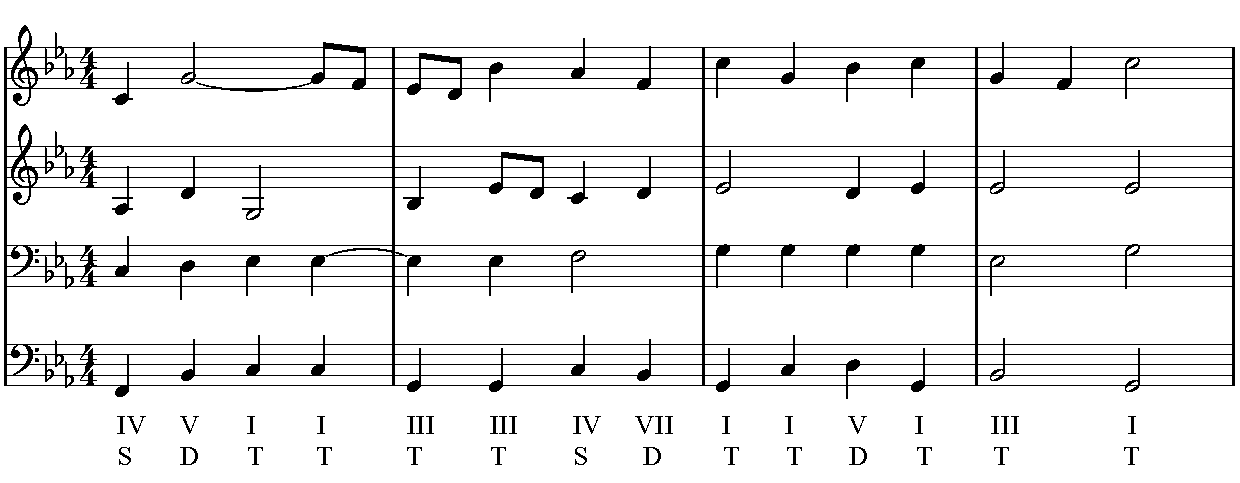
\includegraphics[width=0.9\columnwidth]{Chorale_443576165_minor.pdf}
\caption{Some caption}
\end{figure}

%%%%%%%%%%%%%%%%%%%%%%%%% Conclusion %%%%%%%%%%%%%%%%%%%%%%%%%%%%%%%

\section{Conclusion}

I have presented an application of PTGGs to the topic of automated composition along the sole parameter of rhythm. I detailed one implementation of such a grammar and examined a sample of its output. The grammar shown above is a preliminary attempt, and there are some possible routes for its extension. 

[TODO: need more conclusion]

\subsection{Future Work}

[TODO: rewrite]

One clear choice would be to try introducing rhythmic concepts that this grammar cannot currently express. These include ties, rests, and triple (3/4) meter. The former two items suggest the introduction of more alphabet symbols: a Tied symbol, produced from a Beat or Short, could be interpreted as tied over from the previous note during playback. A Rest symbol could be similarly used to eliminate some articulated notes from the interpreted string. Adding compatibility for triple meter would imply reworking Dotted as a nonterminal symbol.

Another concept that seems to be missing from the current alphabet is that of an embellishment or ornamentation. Such symbols could add short note values before or after more metrically significant beats, and in so doing introduce a third level of metrical hierarchy. A separate way to approach this would be by allowing existing let-in structures in the string to be resolved during or between iterations, rather than at the end of the entire cycle. This would preserve high-level symmetry while allowing for small-scale variations.

With certain adaptations, the proposed grammar could generate rhythms in more contemporary styles: for instance, the composition of mixed-meter passages would require a reworking of the first, Measure-based production phase, and might be better generated additively as opposed to recursively. The grammar already supports the complex and nested tuplets which are often found in classical music of the 20th and 21st centuries, and by slackening the imposed constraint on constant total string duration, it might also be able to generate passages in free meter or “non-geometric” time.

Another direction to explore is context sensitivity. In some cases, it might be helpful to know certain contextual details about a symbol such as: (1) its position within the measure, which typically determines its emphasis (downbeat vs. upbeat), (2) its position within the overall duration of the passage, and (3) whether the passage is increasing or decreasing in rhythmic activity. Otherwise, it is not possible to account for what Schoenberg termed “the tendency of the smallest notes” [10]—a contrapuntal phenomenon wherein shorter durations are used more frequently toward the end of a passage or phrase—without adding other constraints to the rule set.

Finally, these variations and improvements could also be useful for interfacing my grammar with other automated composition algorithms that produce melodies, harmonies, and counterpoint, either by using its output as a blueprint or by including it in a “composition by committee” approach. In that case, it would be important to embed as much contextual and functional knowledge as possible into the alphabet and the symbol parameters so that other grammars and algorithms can make informed decisions. For example, the knowledge that a downbeat is tied over or that two halves of a phrase have some rhythmic symmetry could be interpreted by a harmonic composition algorithm to produce more contextually aware chord sequences.

%%%%%%%%%%%%%%%%%%%%%%%%%%%%%%%%%%%%%%%%%%%%%%%%%%%%%%%%%%%%%%%%%%%%%%%%%%%%%
%bibliography here
\bibliography{musicbib3}

\end{document}
